\begin{abstract}
TODO
\end{abstract}

\chapter{Einleitung}
Schnelles 2D-Rendering ist eine nichttriviale Aufgabe für GPUs. Für viele Anwendungen sind die verfügbaren Bibliotheken im Allgemeinen immer noch viel zu langsam. Um das zu verbessern, haben wir mit \textit{BunnySuite} ein Framework entwickelt, mit dem gängige 2D-Grafik-Bibliotheken einem automatisierten Stresstest ausgesetzt werden können.\\
Mit dem \textit{BunnyMark}\footnote{https://github.com/openfl/openfl-samples/tree/master/demos/BunnyMark} gab es bereits eine Metrik zum Vergleich von Bibliotheken. Jedoch wurde hier nur die Anzahl der gerenderten Objekte (in diesem Fall Häschen, deshalb der Name) gemessen, bei denen noch 60 fps erreicht werden. Diese Zahl war nur schwer zu interpretieren und musste für ein ausführlicheres Ranking durch aussagekräftigere Metriken, bspw. \textit{Renderzeit pro Frame bei X Objekten} ersetzt werden. Auch findet diese Messung bei BunnyMark zu Demozwecken nur interaktiv statt: Häschen werden per Mausklick zur Szene hinzugefügt. Im von uns entwickelten BunnySuite-Framework können solche Messungen automatisiert erfolgen. Die Tests für mehrere Frameworks werden automatisch nacheinander gestartet und das Ergebnis wird in einem Diagramm zusammengefasst. Das Framework ist leicht erweiterbar, so dass man es mit wenig Aufwand an neue Bibliotheken anpassen kann.\\
Das vollautomatisierte Test-Framework soll Entscheidern der Spieleentwicklung die Möglichkeit eines Rankings bieten, um die richtige Bibliothek für ihre Anforderungen zu finden. Des Weiteren sollen Entwickler von Bibliotheken das Framework nutzen können, um ihre eigene Engine zu testen und zu optimieren. Die Leistungen der Bibliotheken können so transparent verglichen werden, was den Wettbewerb zwischen den Bibliotheken stimulieren und Anreize setzen soll, stärker an der Performanz zu arbeiten. 

\chapter{Zeitplan und Aufgabenverteilung}
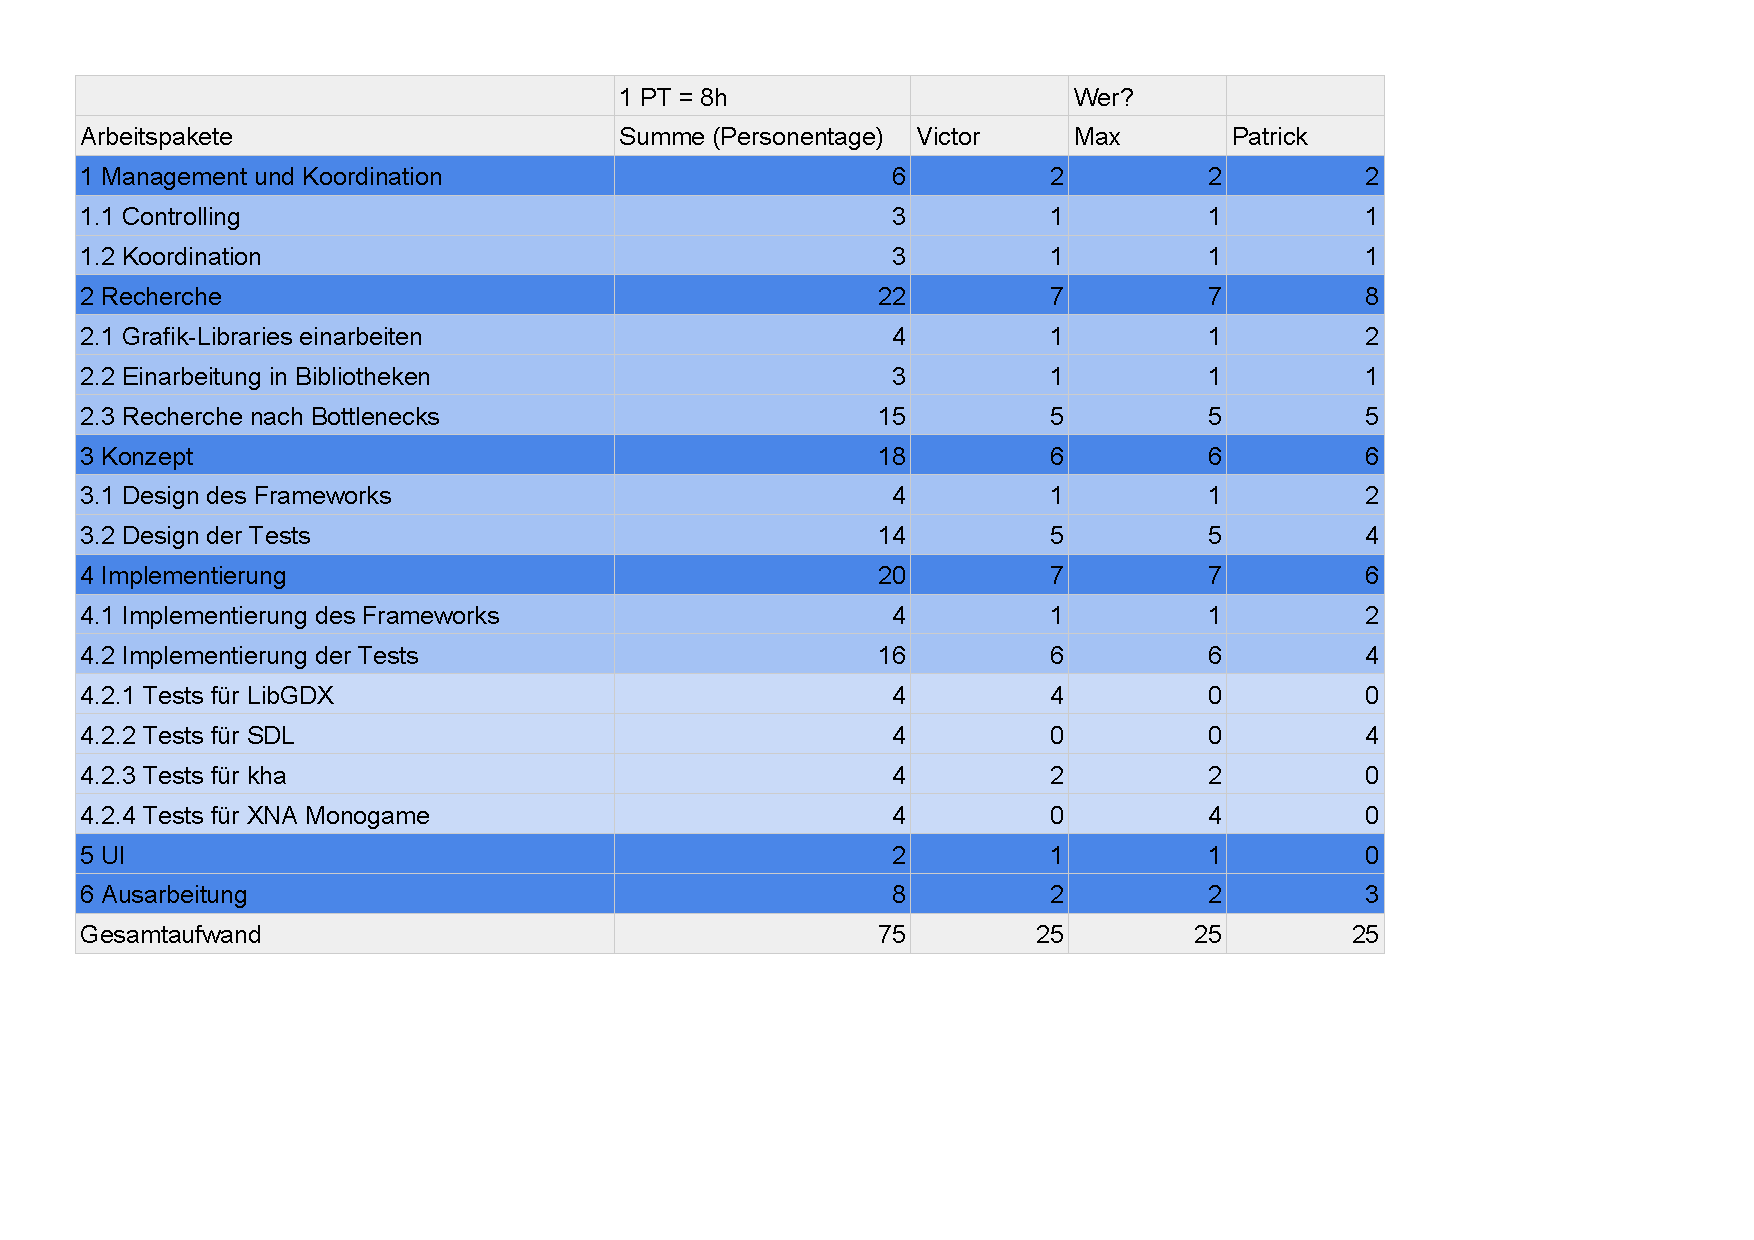
\includegraphics[width=1.2\textwidth]{projektplan.pdf}


\chapter{Grundlagen}
\section{2D-Frameworks}
\section{Benchmarking}
Der Benchmark soll vollautomatisiert erfolgen. Wichtigste Eigenschaft des Benchmarks ist die Vergleichbarkeit der Ergebnisse. Dazu wurde die Renderzeit pro Frame bei X Objekten als Kennzahl eingeführt. Wie bei allen empirischen Untersuchungen muss diese den folgenden drei Kriterien genügen:\\
\begin{description} 
\item[Validität] Dass sich die Kennzahl mit empirischen Messergebnissen deckt, ist garantiert, da sie empirisch zustande kommt. Es wurde die in Entwicklerkreisen übliche Größe {\em Renderzeit pro Frame in Sekunden} gewählt, im Gegensatz zu ihrer Inversen, {\em Frames per Second}, oder einem arbiträren Punktesystem.\\
\item[Objektivität] ist durch die Wohldefiniertheit der einzelnen Testverfahren gegeben (siehe \ref{sec:tests}).\\
\item[Reliabilität] Als Maßnahme für hohe Reliabilität werden alle Messungen jeweils zehn mal durchgeführt und anschließend der Durchschnitt gebildet, um Einflüsse von Hintergrundprozessen zu minimieren. (siehe ..) \\
% Falls es noch eine ausführliche Testreihe zur Reliabilität geben sollte, muss das hier noch eingefügt werden.
\end{description}

\chapter{Konzept und Design}

\section{Allgemeines}
Bei der Konzeption einer Benchmark gibt es grundsätzlich zwei verschiedene Herangehensweisen: Zum einen kann man eine repräsentative, in der Regel sehr komplexe Test-Szene rendern lassen, in der alle möglichen Schwierigkeiten und Bottlenecks vorkommen, die gemeinhin bei der Grafikprogrammierung auftauchen, und damit die GPU an die Grenze der Belastbarkeit zu bringen. Das ist der übliche Ansatz bei im Internet frei verfügbaren Benchmarks\footnote{Ein Beispiel: https://unigine.com/products/benchmarks/heaven/}, die dazu dienen, die Fähigkeiten der eigenen Grafikkarte zu testen. Zum anderen kann man viele einzelne, feingranulare Tests definieren, die auf einzelne Bottlenecks abzielen. Für das BunnySuite-Framework haben wir diese Herangehensweise gewählt, da das Framework explizit für den Vergleich von Grafik-Libraries konzipiert ist. Der Vorteil von feingranularen Tests ist, dass die Ergebnisse für die Entwickler sehr viel aussagekräftiger sind, weil sie ihnen präzise Hinweise geben, an welchen Stellen das eigene Framework hinter die anderen abfällt und wo eine Optimierung am meisten bringen würde. Außerdem vereinfacht dieser Ansatz die Entwicklung und Implementierung der Tests enorm. Ein Nachteil ist, dass die Tests teilweise artifizielle Anforderungen stellen, die in echten 2D-Spielen nicht vorkommen. Dieser Nachteil wird aber dadurch ausgeglichen, dass man die Tests -- soweit sinnvoll -- frei kombinieren kann. Außerdem ist die spätere Erweiterung des Frameworks um komplexere Tests durchaus möglich.

\section{Identifizierte Bottlenecks}
Da jede 2D-Grafik-Bibliothek ihre eigenen Stärken und Schwächen aufweist und für unterschiedliche Zwecke optimiert ist, ist es wichtig, differenzierte Tests durchzuführen, um gezielt mögliche Schwachstellen zu identifizieren, ohne dabei die Stärken zu ignorieren. Zu diesem Zweck wurden verschiedene "Bottlenecks" identifiziert, also häufige Schwachstellen, für die gezielt Tests entwickelt wurden. Diese sind unter anderem:\\
\begin{itemize} 
\item Animieren der Objekte
\item Objekte mit veränderlichen Texturen
\item Vielzahl an gleichzeitig dargestellten Objekten mit unterschiedlichen Texturen
\item Skalierung der Objekte
\item Rotation der Objekte
\item Objekte mit (halb-)transparenten Texturen
\end{itemize}

\chapter{Umsetzung und Tests}

\section{Ablauf der Tests}
Der Ablauf eines Tests im \textit{BunnySuite}-Frameworks ist in Abbildung \ref{dia:architecture} schematisch dargestellt. Das Framework besteht im Wesentlichen aus zwei Teilen: 
\begin{enumerate}
\item Das \textbf{Manager-Skript} ist dafür zuständig, den spezifizierten Test für alle Frameworks nacheinander zu starten, anschließend die Logs zu analysieren und die Ergebnisse in einem Diagramm zu visualisieren.
\item Es gibt eine \textbf{ausführbare EXE-Datei} für jedes Framework. Diese Datei wird vom Manager-Skript gestartet und bekommt die Parameter für die Messung als Argumente über die Command-Line übergeben. Das Programm führt die spezifizierten Tests durch und loggt die Renderzeit pro Frame bei X Objekten.
\end{enumerate}
\begin{figure}[h]
\caption{Ablauf eines Tests}
\centering
\includegraphics[width=0.8\textwidth]{Architecture}
\label{dia:architecture}
\end{figure}
~\\
Der auszuführende Test wird durch folgende Parameter spezifiziert:\\
\begin{description}
\item[test\_name] Der Name eines Tests. Die Tests werden in \ref{sec:tests} aufgelistet.
\item[min\_val] Startwert für die Anzahl X der zu zeichnenden Objekte
\item[max\_val] Endwert für X
\item[step] Schrittweite, um die X nach jeder Messung erhöht wird
\end{description}

\section{Beschreibung der Tests}
\label{sec:tests}

\chapter{Zusammenfassung und Ausblick}

